\documentclass[aspectratio=169]{beamer}

\usetheme[progressbar=frametitle]{metropolis}
\usepackage{appendixnumberbeamer}

\usepackage{booktabs}
\usepackage[scale=2]{ccicons}

\usepackage{pgfplots}
\usepgfplotslibrary{dateplot}

\usepackage{xspace}
\newcommand{\themename}{\textbf{\textsc{metropolis}}\xspace}

\title{Nonparametric Estimation of Matching Efficiency and Mismatch in Labor Markets via Public Employment Security Offices in Japan, 1972-2024}
\date{2024/7/9 Hitotsubashi U}
\subtitle{\textcolor{blue}{Preliminary}}
% \date{\today}

\author{Suguru Oani\\ University of Tokyo Market Design Center (UTMD)}
% \institute{}
%\date{\today}
% \titlegraphic{\hfill\includegraphics[height=1.5cm]{logo.pdf}}

\begin{document}

\maketitle

\section{Introduction}
\begin{frame}{Research Question}
\begin{itemize}
    \item AA
\end{itemize}
\end{frame}

\begin{frame}{Main contributions and findings}
\begin{itemize}
    \item Methodological contribution
    \begin{enumerate}
        \item Examine \textbf{versatility} and \textbf{robustness} of Lange and Papageougeu (2020) and check finite sample performance
        \item Develop \textbf{nonparametric mismatch index,} combining Sahin et al (2014)
    \end{enumerate}
    \item Empirical findings
    \begin{enumerate}
        \item Japanese labor market via Hello Work in 1966-2024
        \begin{enumerate}
            \item Matching Efficiency
            \item Elasticity
        \end{enumerate}
        \item Japanese prefecture-level and industry-level labor market via Hello Work in 2012-2024
        \begin{enumerate}
            \item Matching Efficiency
            \item Elasticity
            \item Mismatch
        \end{enumerate}
    \end{enumerate}
    
\end{itemize}
\end{frame}

\begin{frame}{Related literature}
    \begin{enumerate}
        \item Nonparametric aggregate matching function: Lange\&Papageorgiou (2020, LP)
        \begin{itemize}
            \item Cob Douglass:
            \item -> I examine \textbf{versatility} and \textbf{robustness} of LP via simulation
        \end{itemize}
        \item Mismatch: Şahin, Song, Topa, \& Violante (2014, SSTV)
        \begin{itemize}
            \item Cob Douglass: 
            \item -> I develop \textbf{a nonparametric mismatch index} combining LP with SSTV.
        \end{itemize}
        \item Japanese Labor market
        \begin{itemize}
            \item Cobb Douglass Matching function:
            \item Mismatch:
            \item -> I apply the above method to illustrate long-time and short-time trends of matching efficiency, elasticities, and mismatch.
        \end{itemize}
    \end{enumerate}
\end{frame}

\begin{frame}{Table of contents}
  \setbeamertemplate{section in toc}[sections numbered]
  \tableofcontents%[hideallsubsections]
\end{frame}



\section{Model}

\begin{frame}{Background search model}
\begin{itemize}
    \item Background search model
    \item $(U,V,A)$
\end{itemize}
    
\end{frame}


\begin{frame}{Aggregate matching function}
\begin{itemize}
    \item Aggregate matching function $m$ is defined as
    \begin{align*}
        H=m(AU,V)
    \end{align*}
    where $H$ is the number of hires and $m$ satisfies two conditions:
    \begin{enumerate}
        \item \textbf{Constant returns to scale (CRS)}
        \begin{itemize}
            \item Cobb Douglass: $m=AU^{\alpha}V^{1-\alpha}$ with vacancy share $\alpha$
        \end{itemize}
        \item $U\perp A|V$, i.e., \textbf{independence between $U$ and $A$ conditional on $V$}
    \end{enumerate}
    
        \item Our goal is to \textbf{recover unobserved $A$ from observed $(H,U,V)$.}
\end{itemize}
    
\end{frame}

\begin{frame}{Mismatch}
    \begin{itemize}
    \item [TBA]
\end{itemize}
\end{frame}


\begin{frame}{Why nonparametric is better than Cobb Douglass with fixed effects?}
\begin{itemize}
    \item Suppose that we observe $M$ markets in $T$ years.
    \item Cobb Douglass specification estimates $T+M+1$ parameters.
    \begin{itemize}
        \item $T$ year fixed effects.
        \item $M$ market fixed effects.
        \item constant vacancy share parameter $\alpha$.
    \end{itemize}
    \item Nonparametric approach estimates $T\times M$ efficiencies corresponding time-varying elasticities.
    \item Trade-off: \textbf{``Much more" flexibility vs sample size}
    \begin{itemize}
        \item We want to check finite sample performance.
    \end{itemize}
\end{itemize}
    
\end{frame}



\section{Identification and Estimation}

\begin{frame}{Intuition}
    \begin{itemize}
    \item Two urns example.
    \end{itemize}
\end{frame}

\begin{frame}{Nonparametric identification}
    \begin{itemize}
    \item Applying Matzkin (2003), LP shows that XX
    \end{itemize}
\end{frame}

\begin{frame}{Nonparametric estimation}
    \begin{itemize}
    \item [TBA]
    \end{itemize}
\end{frame}



\section{Monte Carlo simulation results}

\begin{frame}{Motivation for finite sample performance}
\begin{itemize}
    \item We want to check \textbf{robustness} to specification, stationarity, and endogeneity.
    \begin{enumerate}
        \item Restricting CRS class including Cobb Douglas
        \item Experiment stationary ARIMA(1,0,0) and nonstationary ARIMA(0,1,0)
        \item Check robustness to violation of independence of $A$ and $U$ conditional on $V$
    \end{enumerate}
    \item We want to confirm how large enough the sample size is.
    \item We want to quantify the bias of the standard Cobb Douglass specification \textcolor{blue}{[Skipped]}
\end{itemize}
    
\end{frame}

\begin{frame}{Setup: DGP}
\begin{itemize}
    \item sample size $T=50,100, 200$
    \item CRS class specification of $m$
    \begin{itemize}
        \item Cobb Douglas
        \item Perfect substitute
    \end{itemize}
    \item stationarity of $(A,U,V)$
    \begin{itemize}
        \item ARIMA(1,0,0)
        \item ARIMA(0,1,0)
    \end{itemize}
    \item endogeneity of $(A,U,V)$
    \item Other tuning parameter: kernel choice and bandwidth  \textcolor{blue}{[Now fixed]}
    \item  \textcolor{blue}{Formal Monte Carlo simulation table is under construction}
\end{itemize}
    
\end{frame}

\begin{frame}{Illustrative fitting plot: Sample size}
\begin{itemize}
    \begin{figure}[!ht]
  \begin{center}

  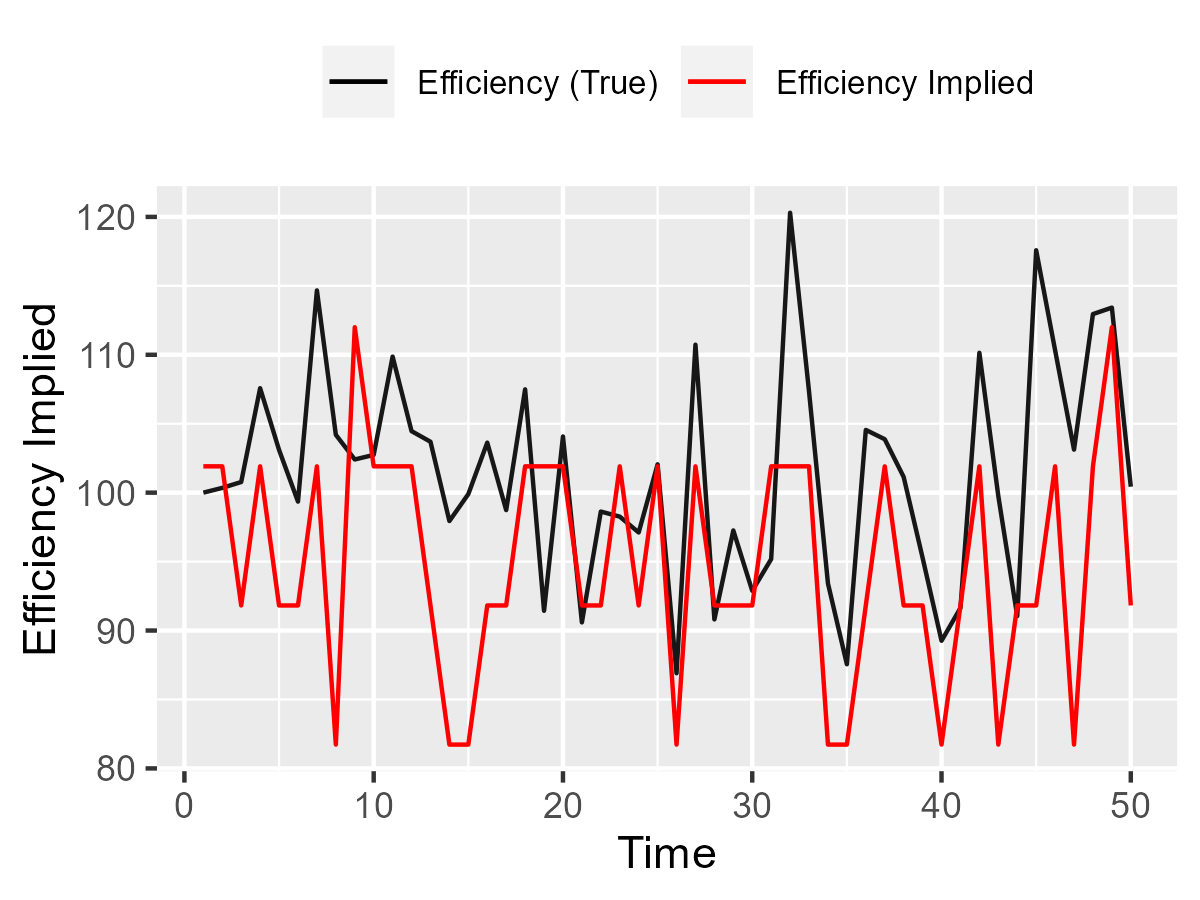
\includegraphics[width = 0.37\textwidth]
  {figuretable/illustrative_plot_implied_efficiency_num_time_50_cobb_douglas_0.3_AR1_I0.png}
  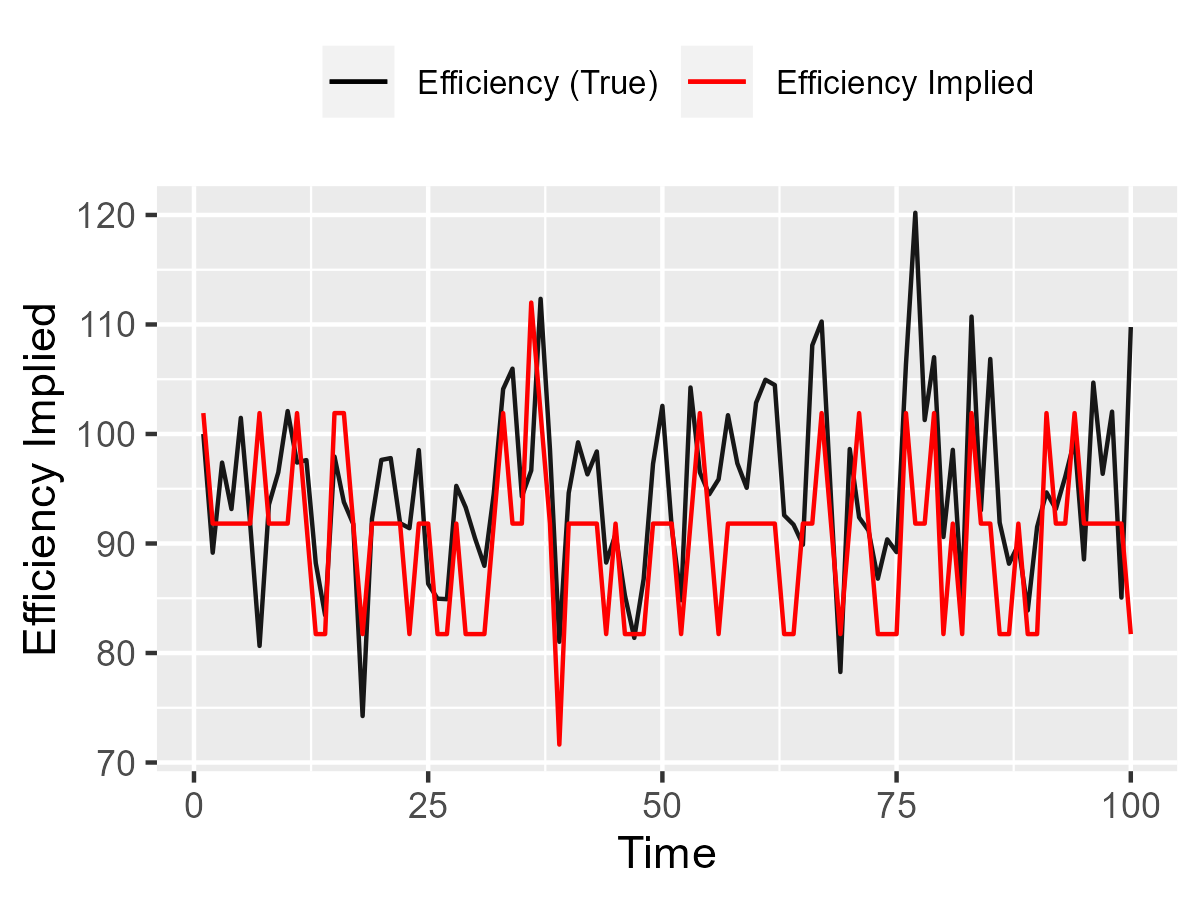
\includegraphics[width = 0.37\textwidth]
  {figuretable/illustrative_plot_implied_efficiency_num_time_100_cobb_douglas_0.3_AR1_I0.png}
  \end{center}
  \footnotesize
  %Note: 
\end{figure} 
\item Pick one simulation path.
\item $T=100$ seems enough.
\end{itemize}
\end{frame}

\begin{frame}{Illustrative fitting plot: With and without stationary}
\begin{itemize}
    \item TBA
    \begin{figure}[!ht]
  \begin{center}

  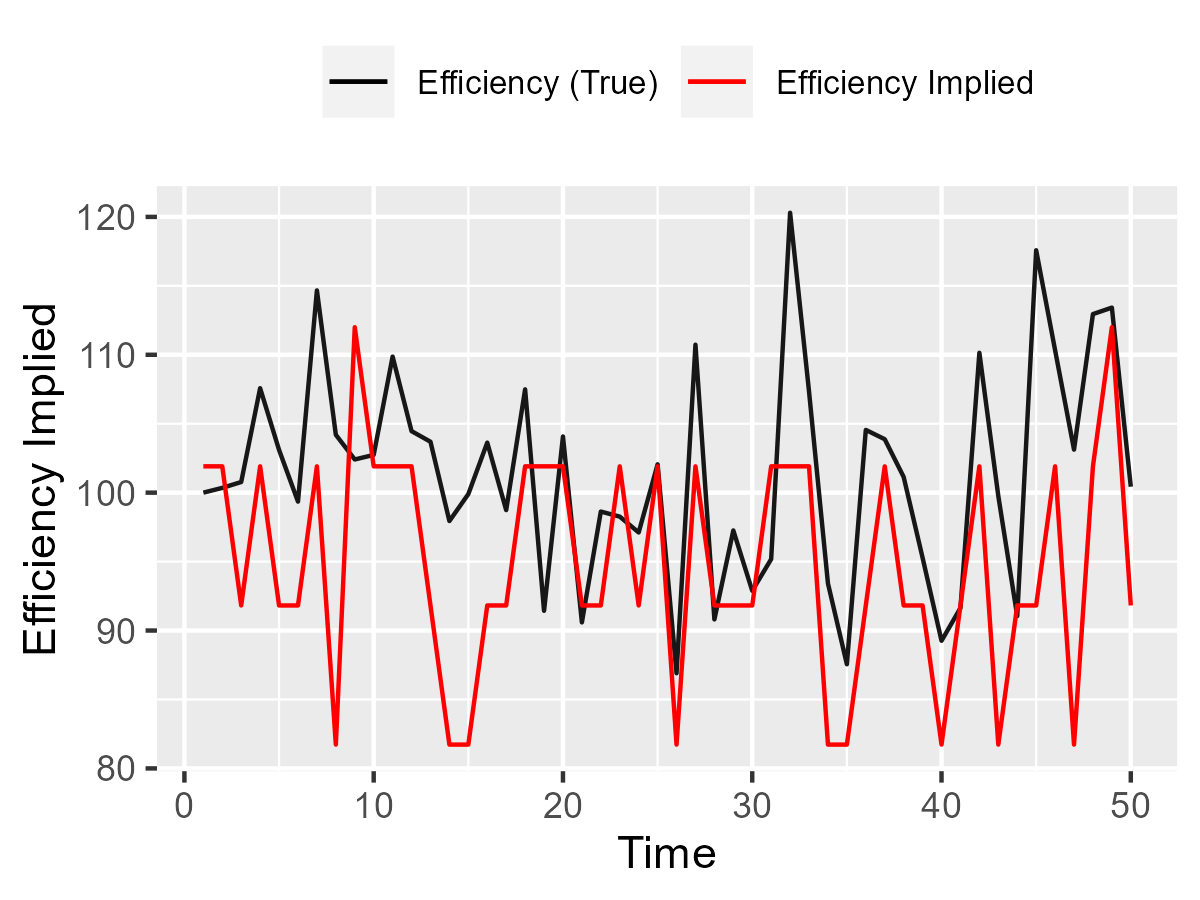
\includegraphics[width = 0.37\textwidth]
  {figuretable/illustrative_plot_implied_efficiency_num_time_50_cobb_douglas_0.3_AR1_I0.png}
  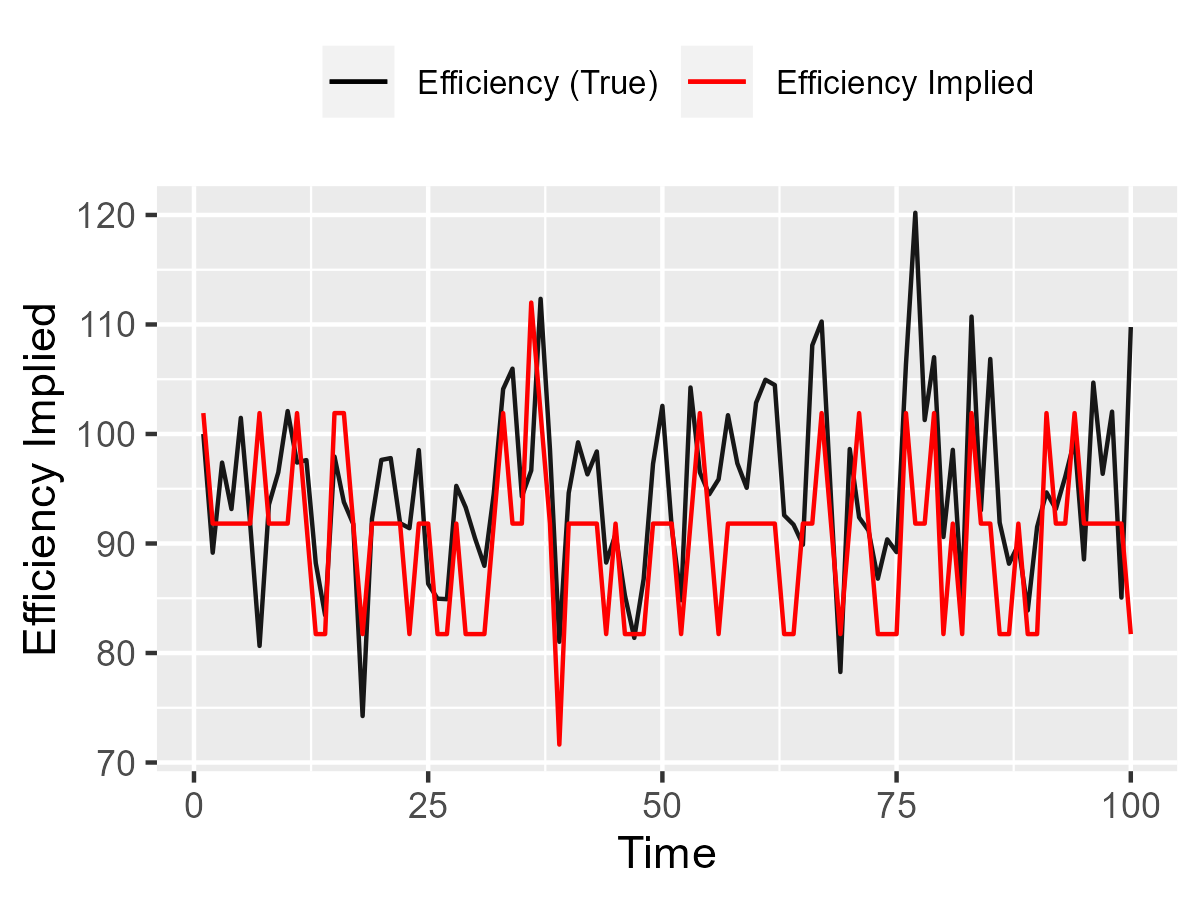
\includegraphics[width = 0.37\textwidth]
  {figuretable/illustrative_plot_implied_efficiency_num_time_100_cobb_douglas_0.3_AR1_I0.png}
  \end{center}
  \footnotesize
  %Note: 
\end{figure} 
\end{itemize}
\end{frame}

\begin{frame}{Illustrative fitting plot: With and without endogeneity}
\begin{itemize}
    \item TBA
    \begin{figure}[!ht]
  \begin{center}

  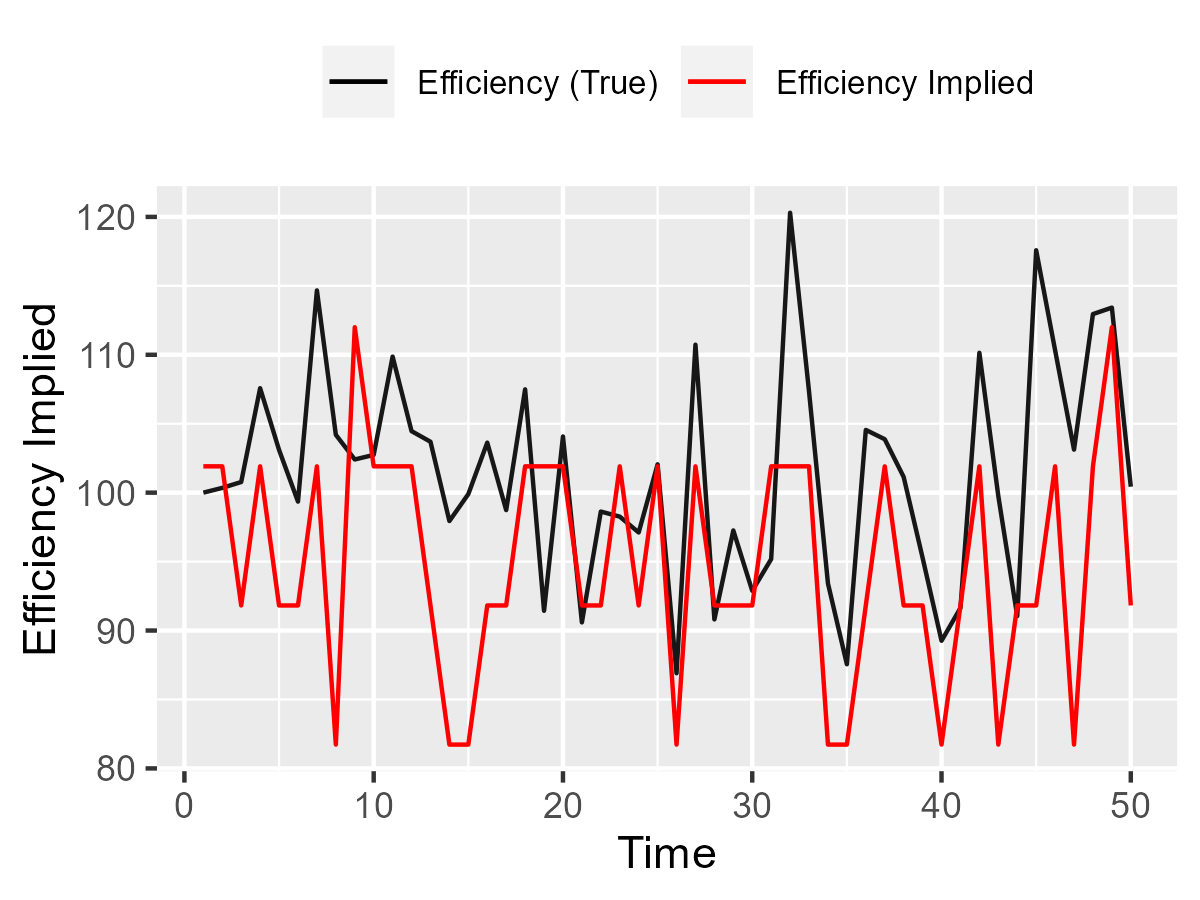
\includegraphics[width = 0.37\textwidth]
  {figuretable/illustrative_plot_implied_efficiency_num_time_50_cobb_douglas_0.3_AR1_I0.png}
  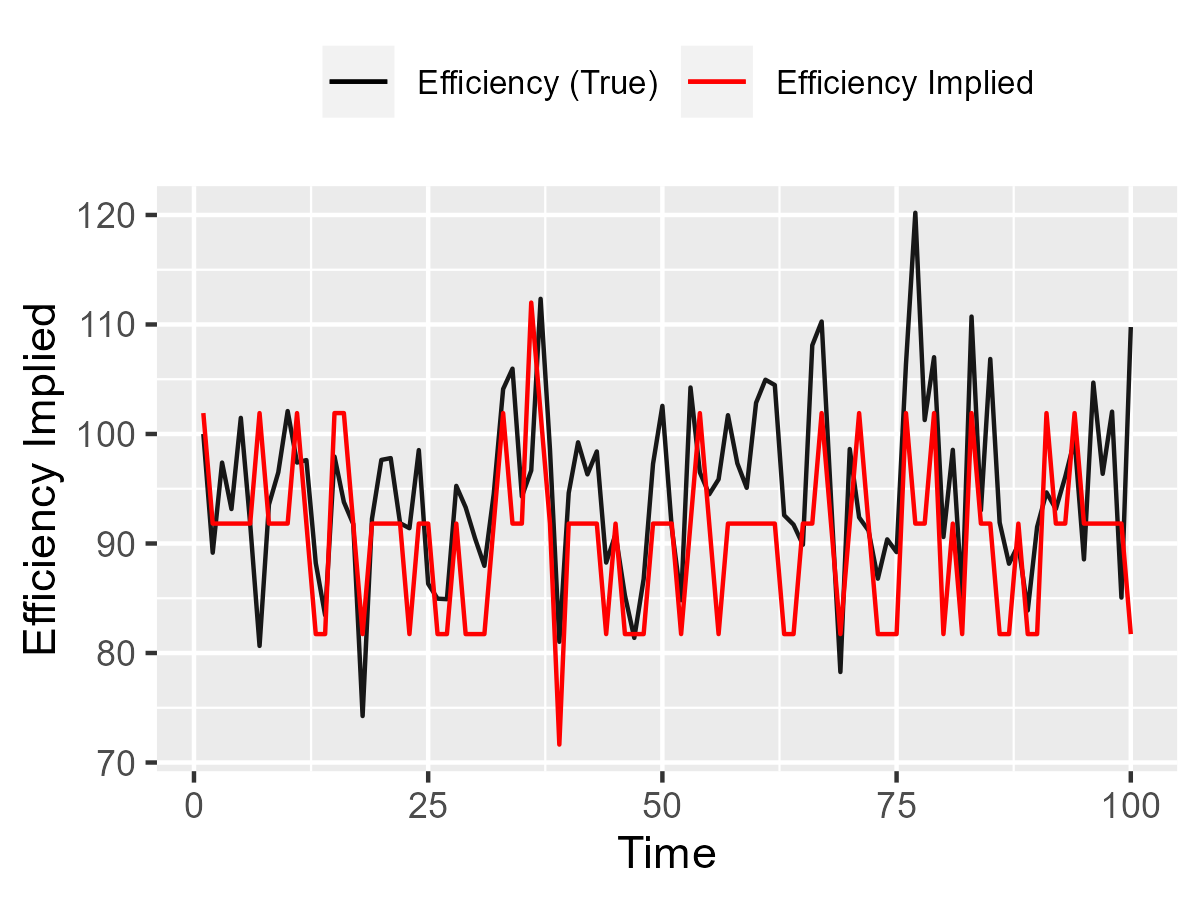
\includegraphics[width = 0.37\textwidth]
  {figuretable/illustrative_plot_implied_efficiency_num_time_100_cobb_douglas_0.3_AR1_I0.png}
  \end{center}
  \footnotesize
  %Note: 
\end{figure} 
\end{itemize}
\end{frame}

% \begin{frame}{Monte Carlo simulation results}
% \begin{itemize}
%     \item TBA
%     \item Specification 1: each cell shows IMSE
%     \begin{itemize}
%         \item X axis $T=10,20,30,40,50,100$ 
%         \item Y1 axis stationarity level
%         \item Y2 axis endogeneity level
%     \end{itemize}
%     \item Specification 2: each cell shows IMSE
%     \begin{itemize}
%         \item X axis $T=10,20,30,40,50,100$ 
%         \item Y1 axis stationarity level
%         \item Y2 axis endogeneity level
%     \end{itemize}
    
% \end{itemize}
    
% \end{frame}


\section{Data}

\begin{frame}{Data}
  \begin{itemize}
      \item Hello Work data
  \end{itemize}
\end{frame}



\section{Empirical Results: 1966-2023}


\begin{frame}{Overview of the first empirical exercise}
    \begin{itemize}
        \item Data: Country-year-level data in 1966-2023.
        \item Estimate matching efficiency for each dataset
        \begin{enumerate}
            \item All (=Full-time + Part-time)
            \item Decompose Full-time and Part-time
        \end{enumerate}
    \end{itemize}
\end{frame}

\begin{frame}{Residual plot}
    \begin{figure}[!ht]
  \begin{center}
  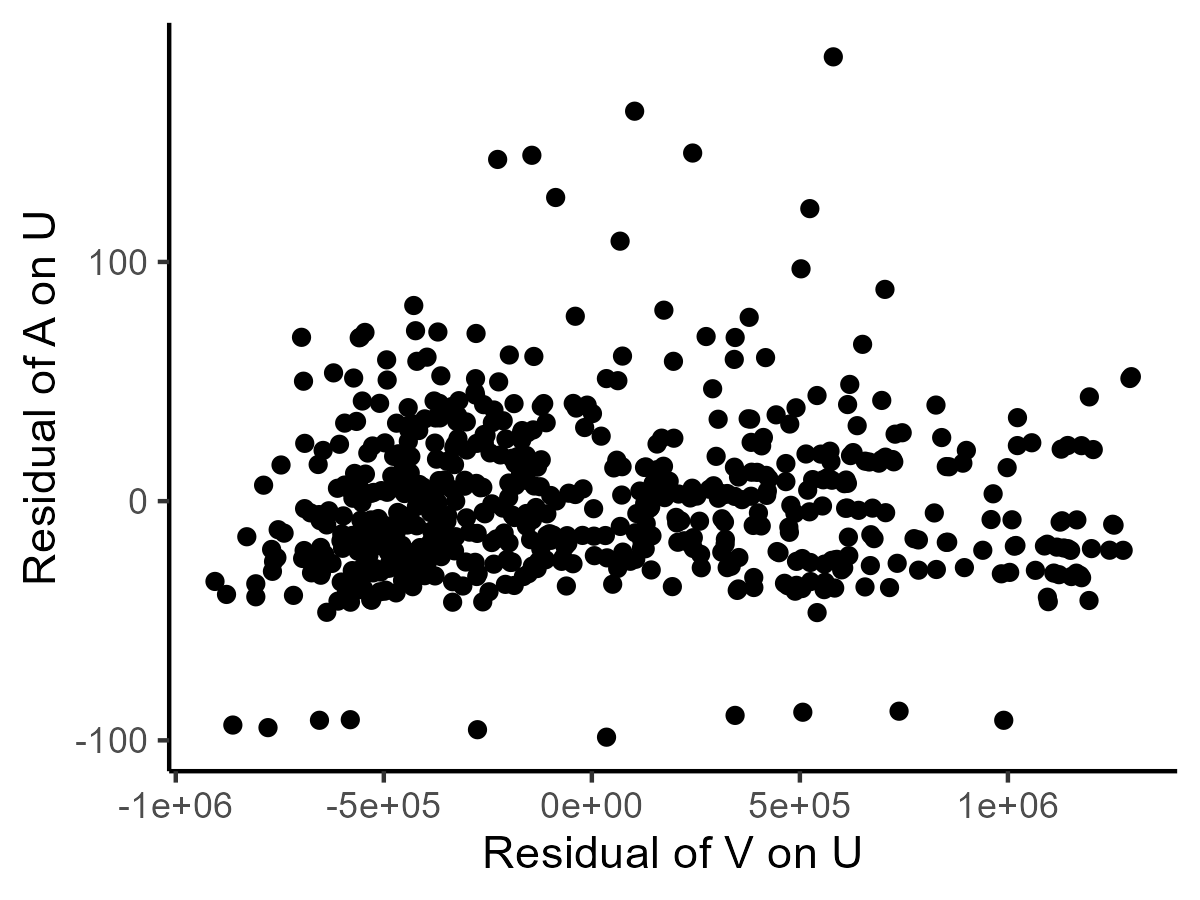
\includegraphics[width = 0.50\textwidth]
  {figuretable/residual_plot_month_aggregate.png}
  \end{center}
  \footnotesize
  %Note: 
\end{figure} 
\begin{itemize}
    \item A
\end{itemize}
\end{frame}



\begin{frame}{$U,V,H$ and Tightness $V/U$}
    \begin{figure}[!ht]
  \begin{center}
  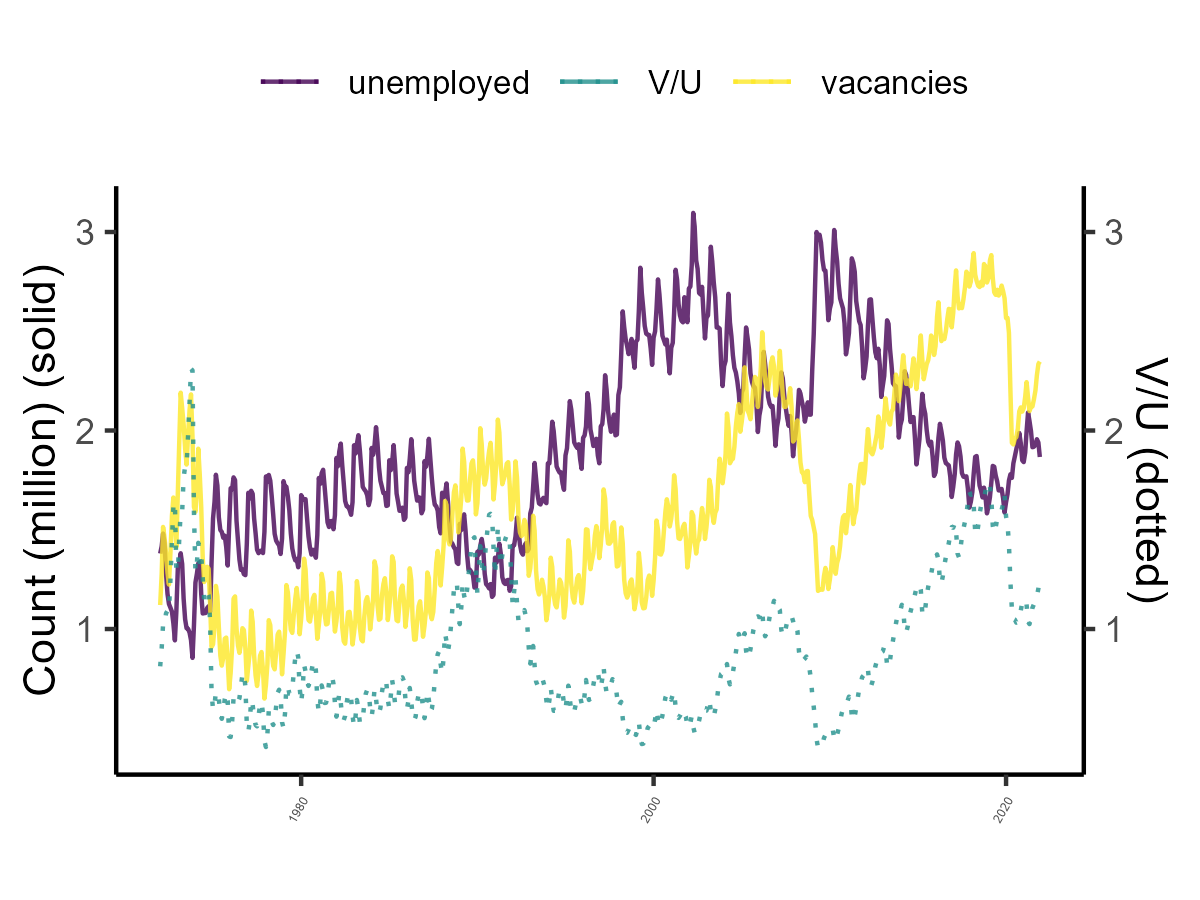
\includegraphics[width = 0.37\textwidth]
  {figuretable/unemployed_vacancy_month_aggregate.png}
  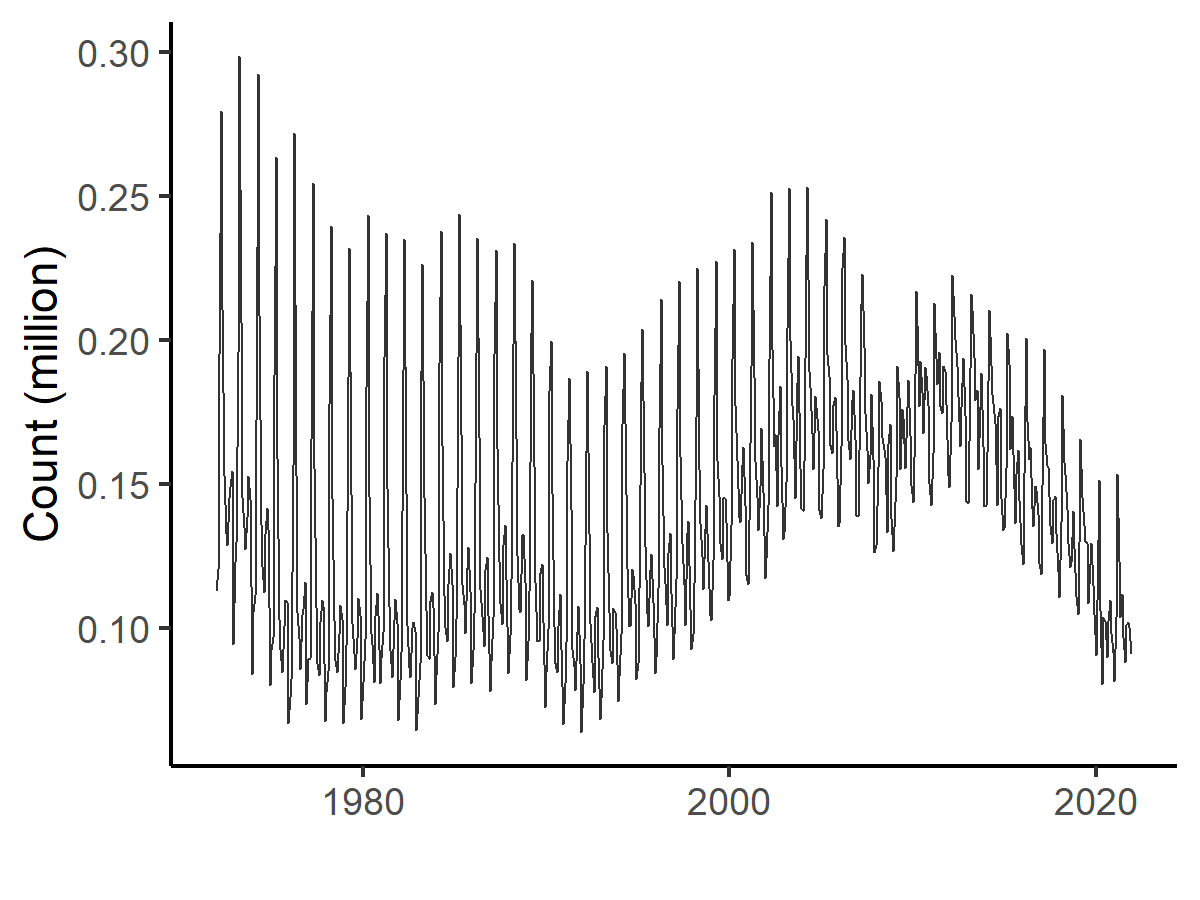
\includegraphics[width = 0.37\textwidth]
  {figuretable/hire_month_aggregate.png}
  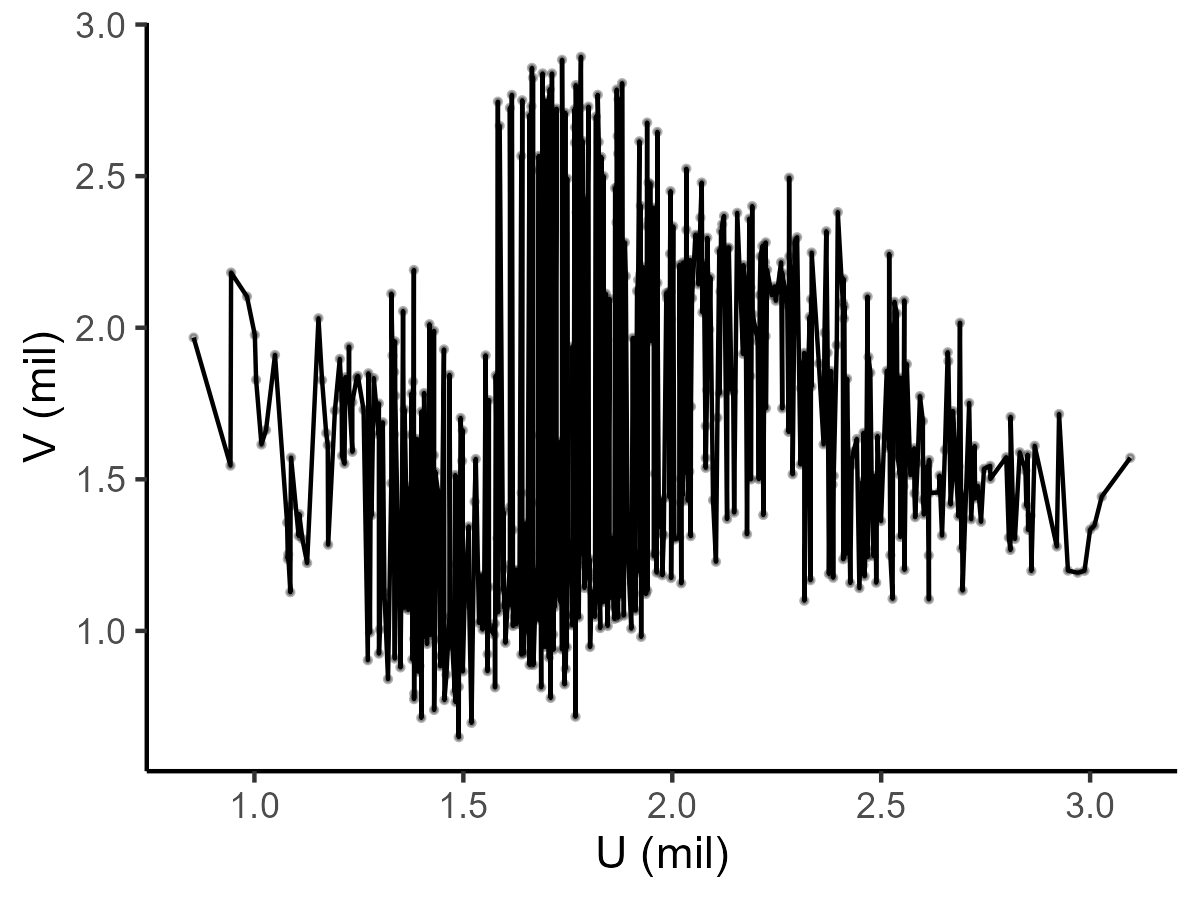
\includegraphics[width = 0.37\textwidth]
  {figuretable/unemployed_vacancies_berveridge_month_aggregate.png}
  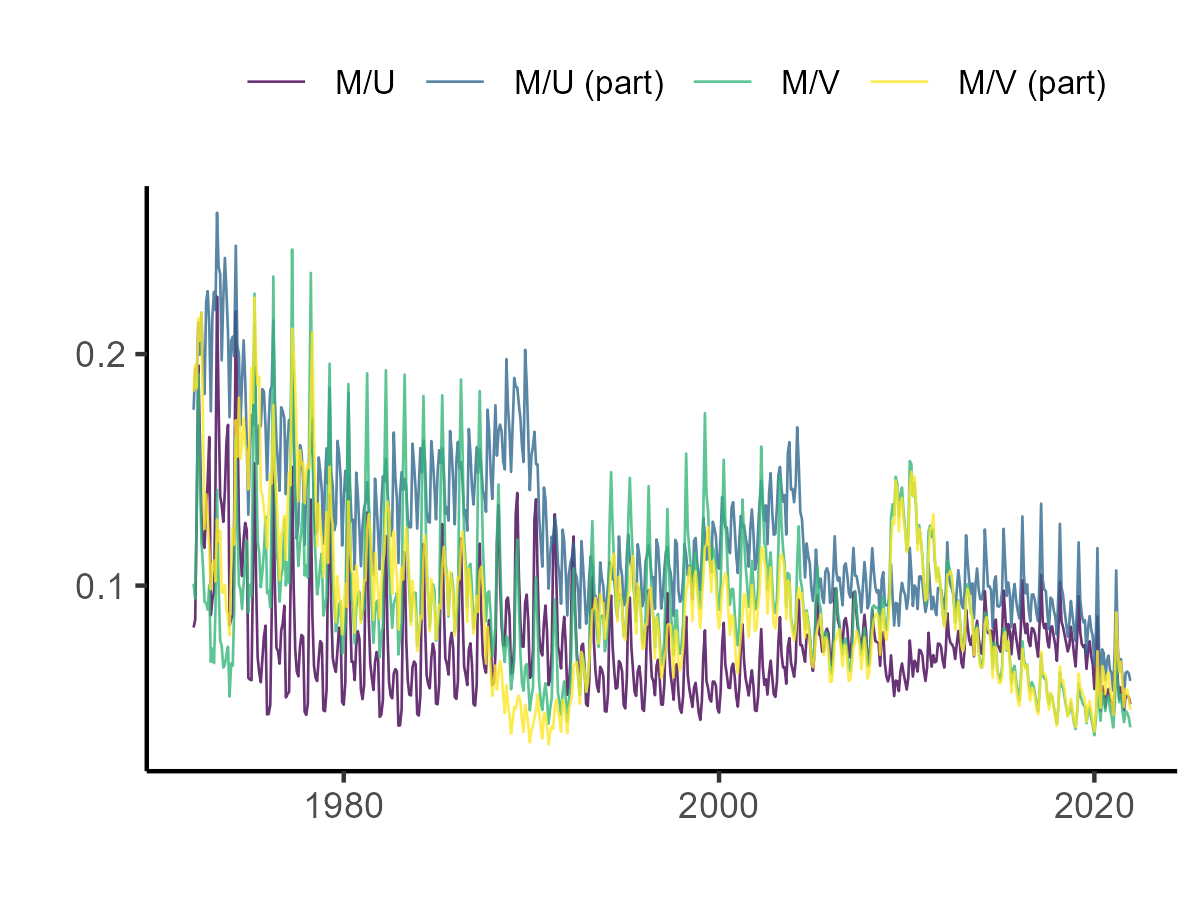
\includegraphics[width = 0.37\textwidth]
  {figuretable/job_finding_rate_worker_finding_rate_month_aggregate.png}
  \end{center}
  \footnotesize
  %Note: 
\end{figure} 
\begin{itemize}
    \item A
\end{itemize}
\end{frame}

\begin{frame}{Matching Efficiency and Elasticities}
    \begin{figure}[!ht]
  \begin{center}
  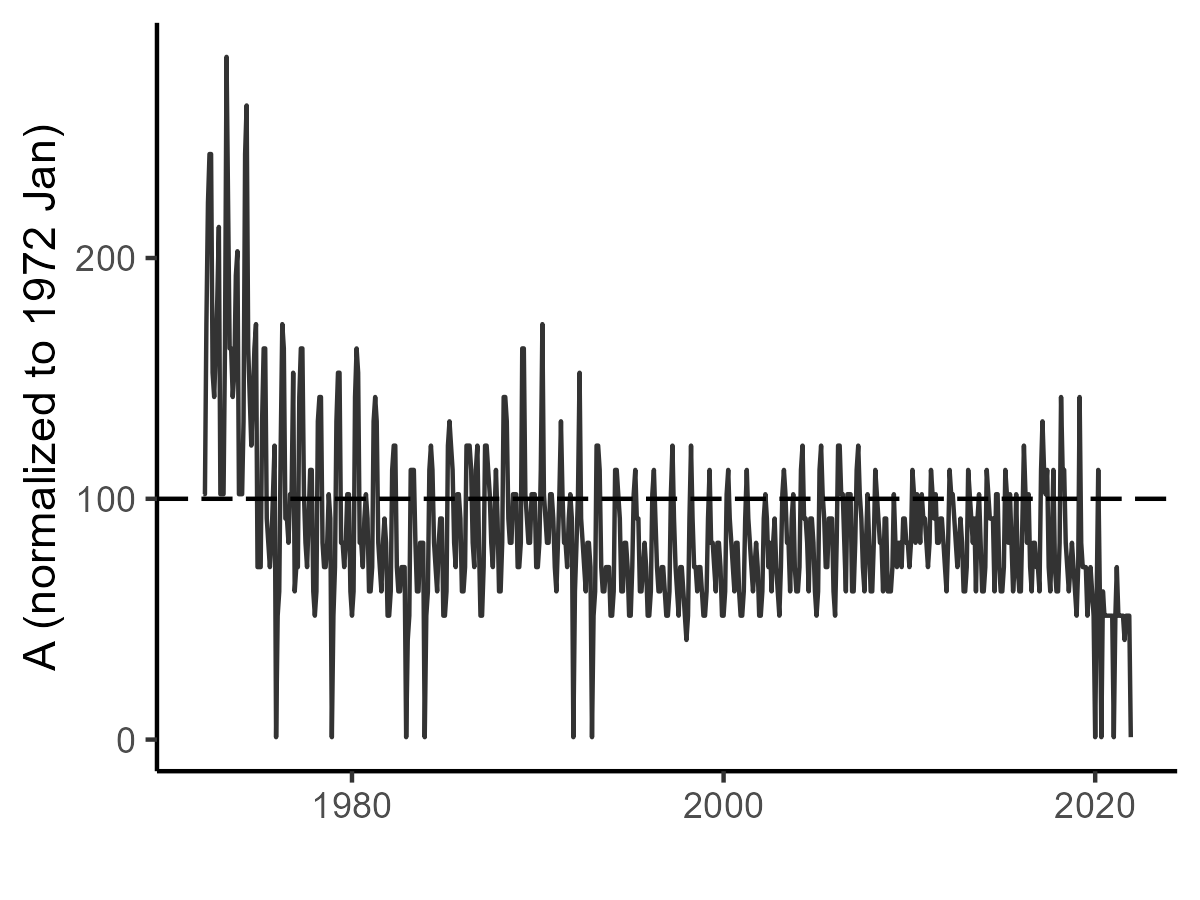
\includegraphics[width = 0.37\textwidth]
  {figuretable/matching_efficiency_month_aggregate.png}
  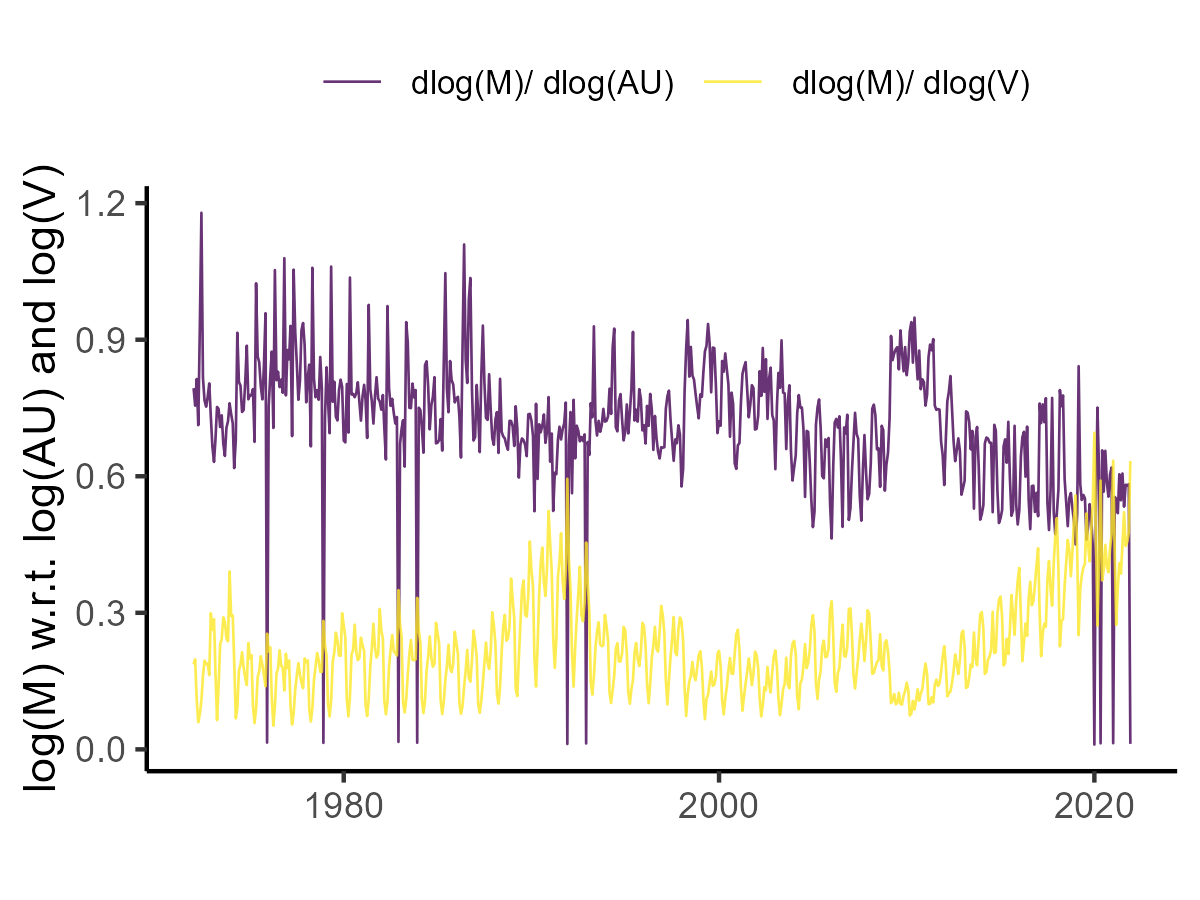
\includegraphics[width = 0.37\textwidth]
  {figuretable/elasticity_month_aggregate.png}
  \end{center}
  \footnotesize
  %Note: 
\end{figure} 
\begin{itemize}
    \item A
\end{itemize}
\end{frame}

\begin{frame}{Correlation of Efficiency and Tightness}
    \begin{figure}[!ht]
  \begin{center}
  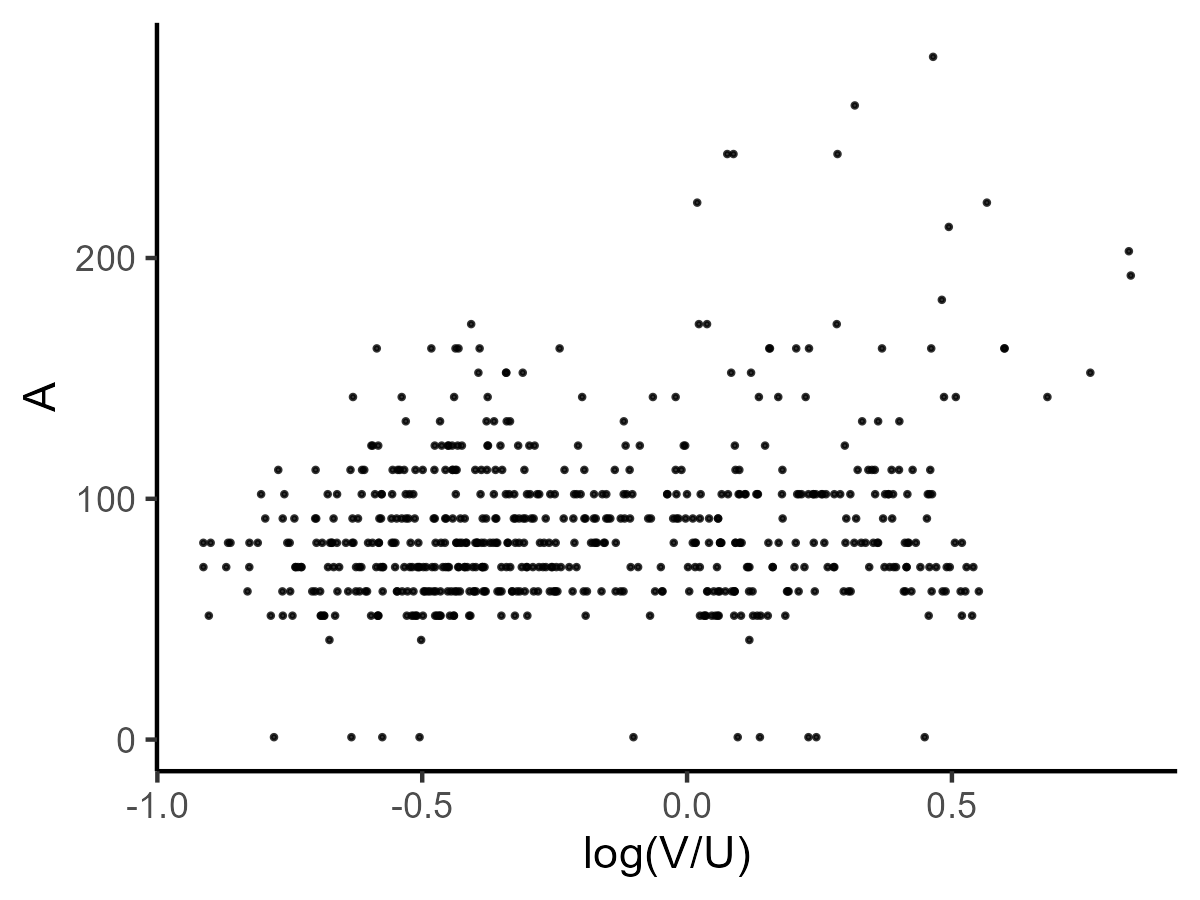
\includegraphics[width = 0.37\textwidth]
  {figuretable/efficiency_tightness_plot_month_aggregate.png}
  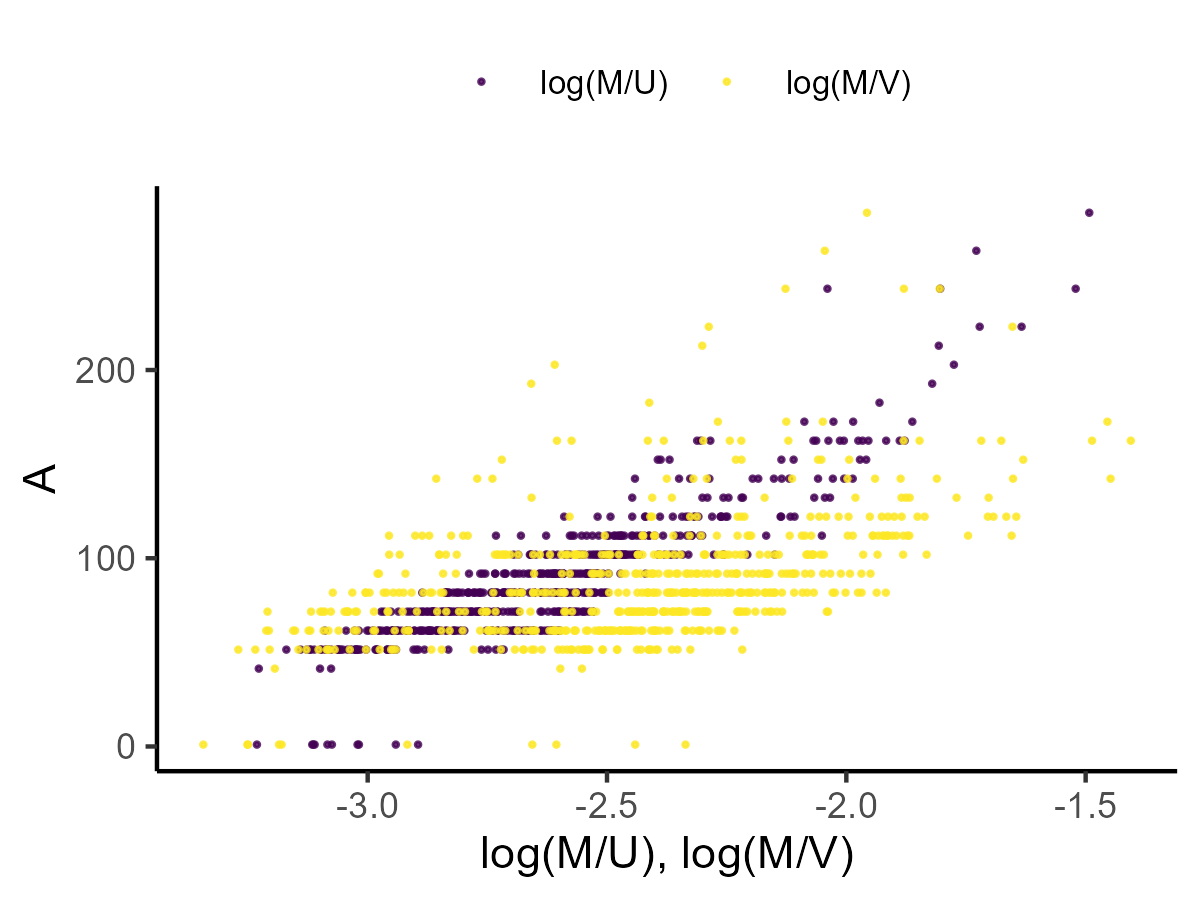
\includegraphics[width = 0.37\textwidth]
  {figuretable/job_finding_rate_efficiency_plot_month_aggregate.png}
  \end{center}
  \footnotesize
  %Note: 
\end{figure} 
\begin{itemize}
    \item A
\end{itemize}
\end{frame}



\begin{frame}{$U,V,H$ and Tightness $V/U$ (Full-time and Part-time)}
    \begin{figure}[!ht]
  \begin{center}
  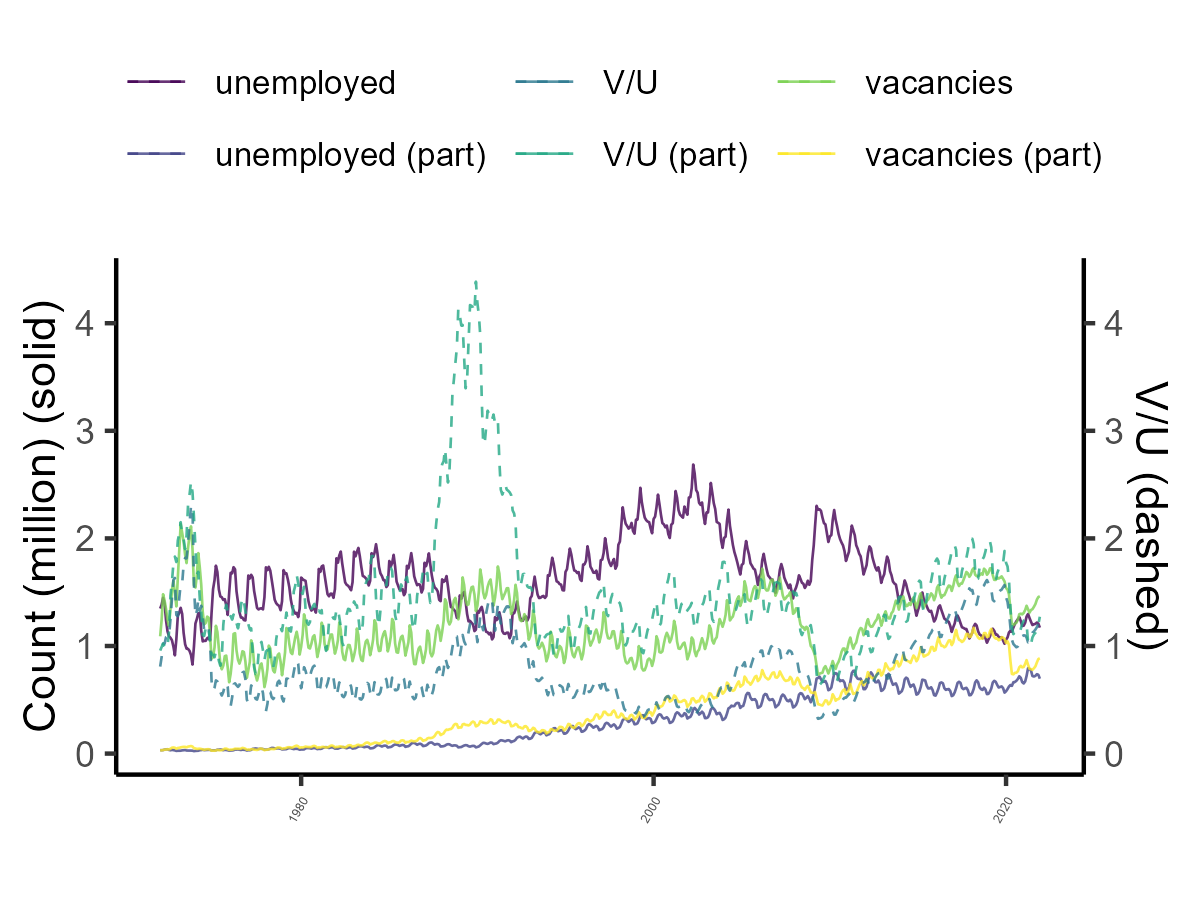
\includegraphics[width = 0.3\textwidth]
  {figuretable/unemployed_vacancy_month_full_time_part_time.png}
  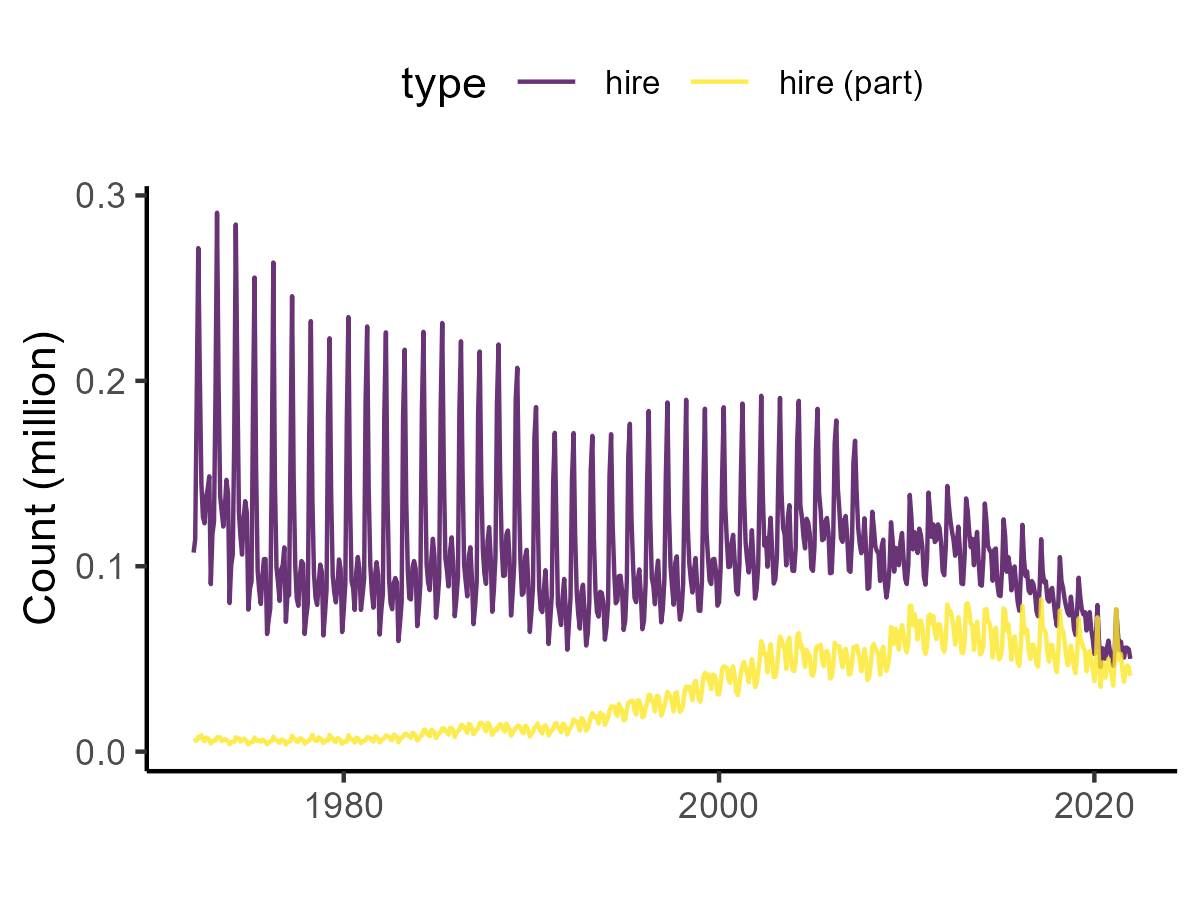
\includegraphics[width = 0.3\textwidth]
  {figuretable/hire_month_full_time_part_time.png}
  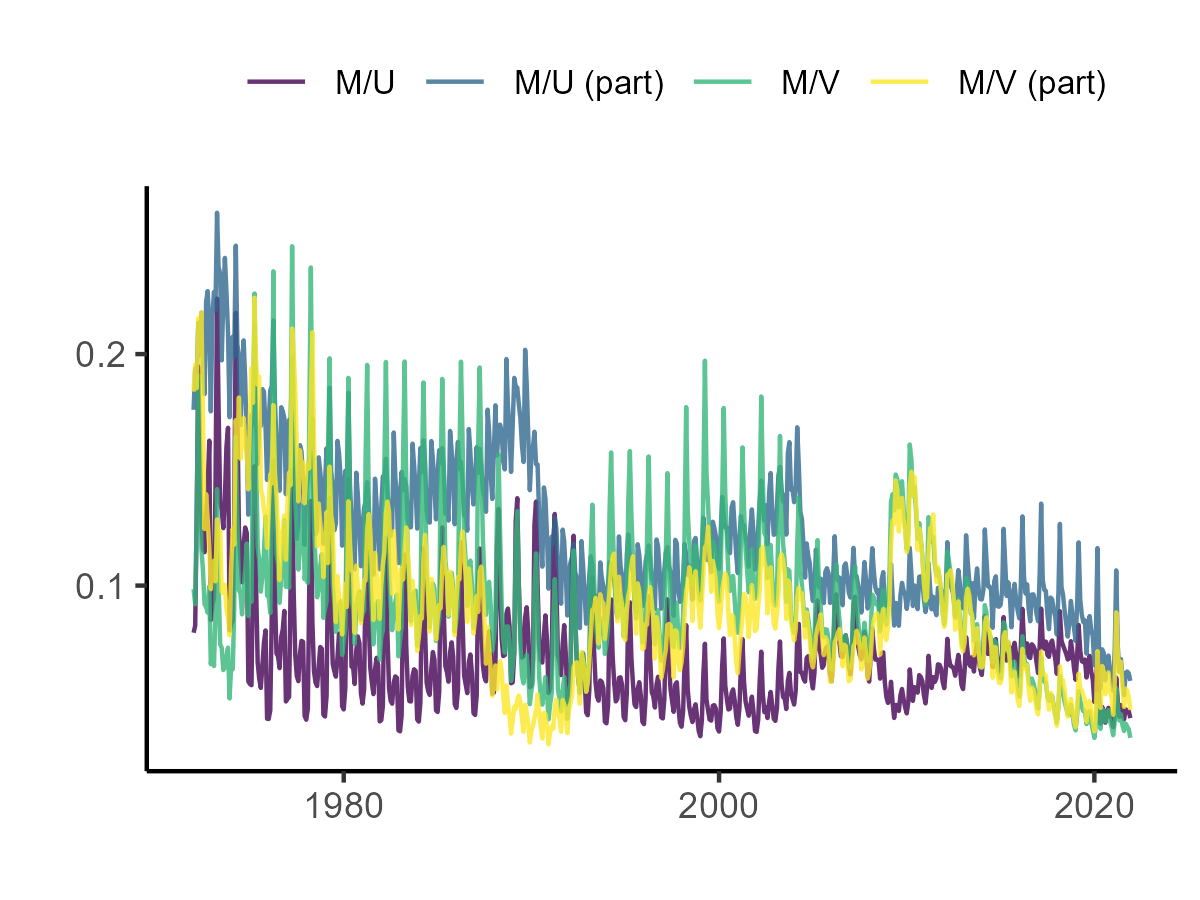
\includegraphics[width = 0.3\textwidth]
  {figuretable/job_finding_rate_worker_finding_rate_month_full_time_part_time.png}
  \end{center}
  \footnotesize
  %Note: 
\end{figure} 
\begin{itemize}
    \item A
\end{itemize}

\end{frame}

\begin{frame}{Matching Efficiency and Elasticities (Full-time and Part-time)}
    \begin{figure}[!ht]
  \begin{center}
  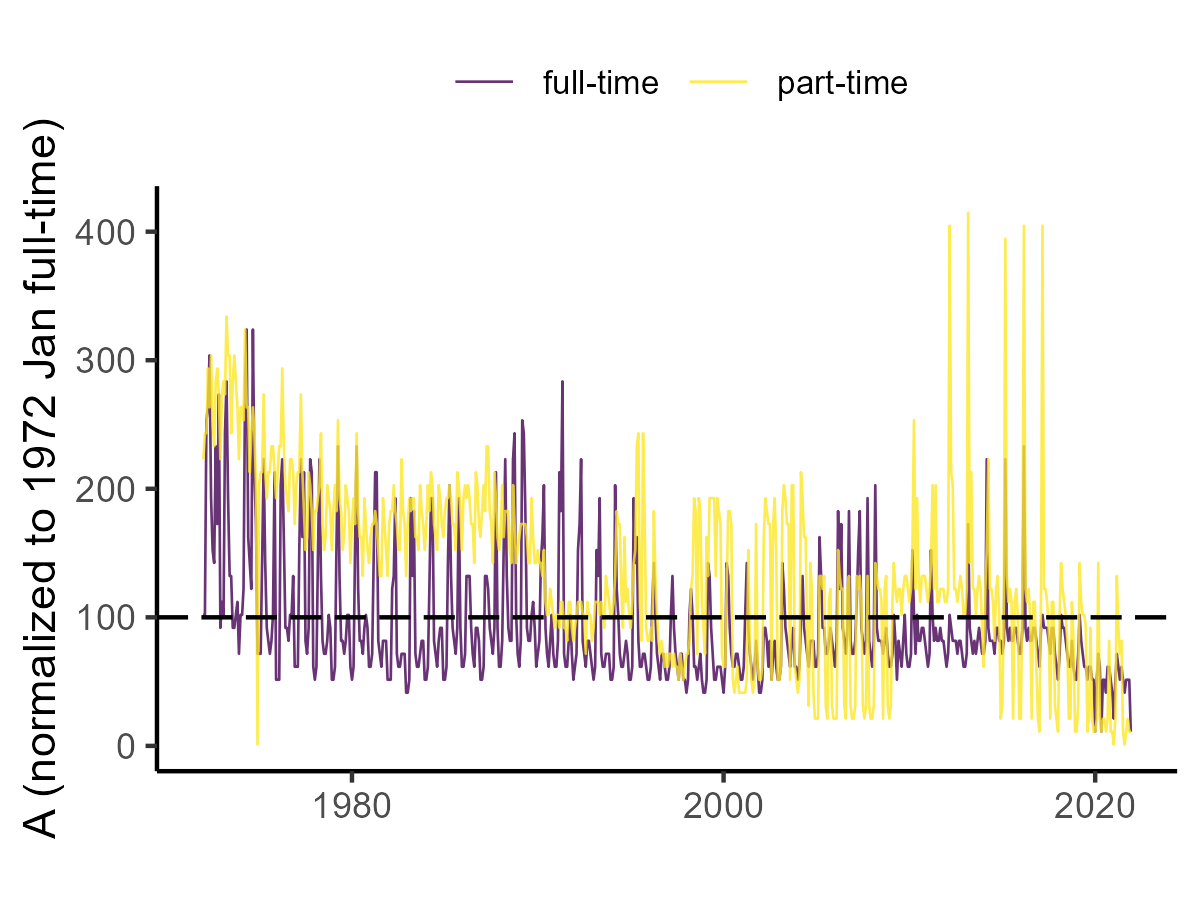
\includegraphics[width = 0.37\textwidth]
  {figuretable/matching_efficiency_month_full_time_part_time.png}
  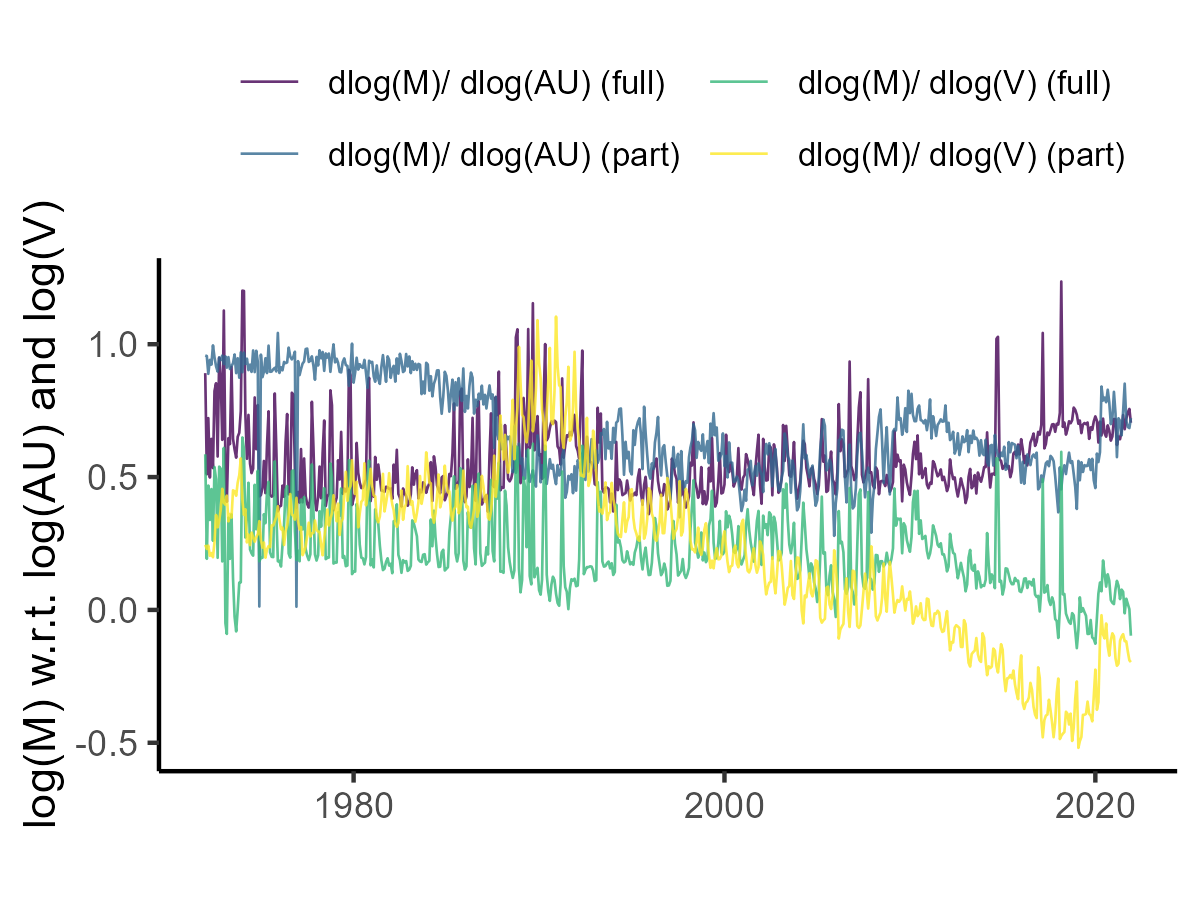
\includegraphics[width = 0.37\textwidth]
  {figuretable/elasticity_month_full_time_part_time.png}
  \end{center}
  \footnotesize
  %Note: 
\end{figure} 

\begin{itemize}
    \item A
\end{itemize}
\end{frame}

\begin{frame}{Correlation of Efficiency and Tightness (Full-time and Part-time)}
    
\begin{figure}[!ht]
  \begin{center}
  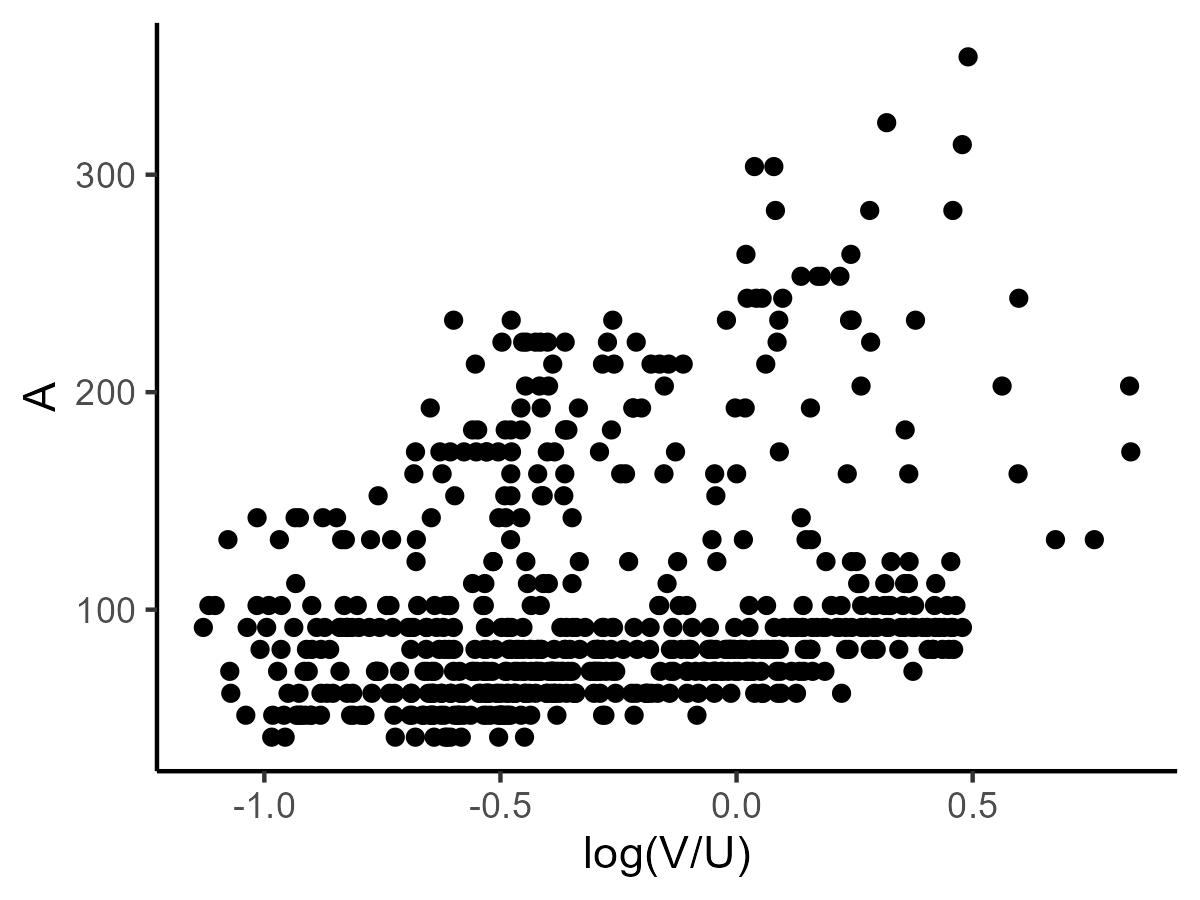
\includegraphics[width = 0.37\textwidth]
  {figuretable/efficiency_tightness_plot_month_full_time.png}
  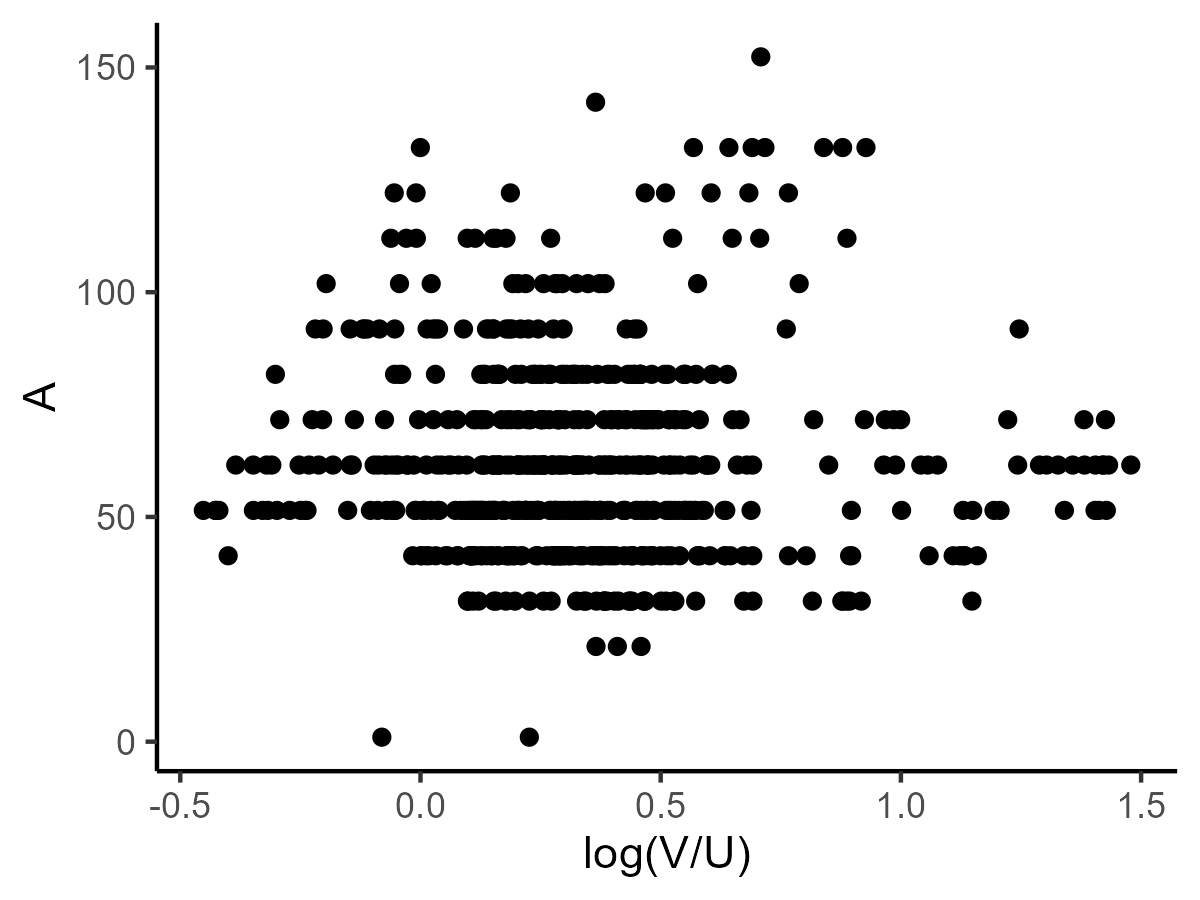
\includegraphics[width = 0.37\textwidth]
  {figuretable/efficiency_tightness_plot_month_part_time.png}
  \end{center}
  \footnotesize
  %Note: 
\end{figure} 
\begin{itemize}
    \item A
\end{itemize}
\end{frame}

\begin{frame}{Summary of long time trends}
    \begin{itemize}
        \item Matching efficiency sharply declines after 2015 by 50 \% relative to 1966.
        \begin{itemize}
            \item Seemingly driven by full-time's efficiency decline.
        \end{itemize}
        
        \item Matching efficiency and Tightness are positively correlated.
        \begin{itemize}
            \item Full-time has a stronger correlation.
        \end{itemize}
        
    \end{itemize}
\end{frame}

\section{Empirical Results: 2012-2024}

\begin{frame}{Overview of the second empirical exercise}
    \begin{itemize}
        \item Data: Prefecture-month-level and industry-month-level data in 2012-2023.
        \item Estimate matching efficiency for each dataset
        \begin{enumerate}
            \item All (=Full-time + Part-time)
            \item Decompose Full-time and Part-time \textcolor{blue}{[Skipped]}
        \end{enumerate}
        \item Compute nonparametric mismatch index across prefectures and industries
        \begin{enumerate}
            \item All (=Full-time + Part-time)
            \item Decompose Full-time and Part-time \textcolor{blue}{[Skipped]}
        \end{enumerate}
    \end{itemize}
\end{frame}

\begin{frame}{Matching Efficiency: Tohoku and Kanto}
\begin{figure}[!ht]
  \begin{center}

  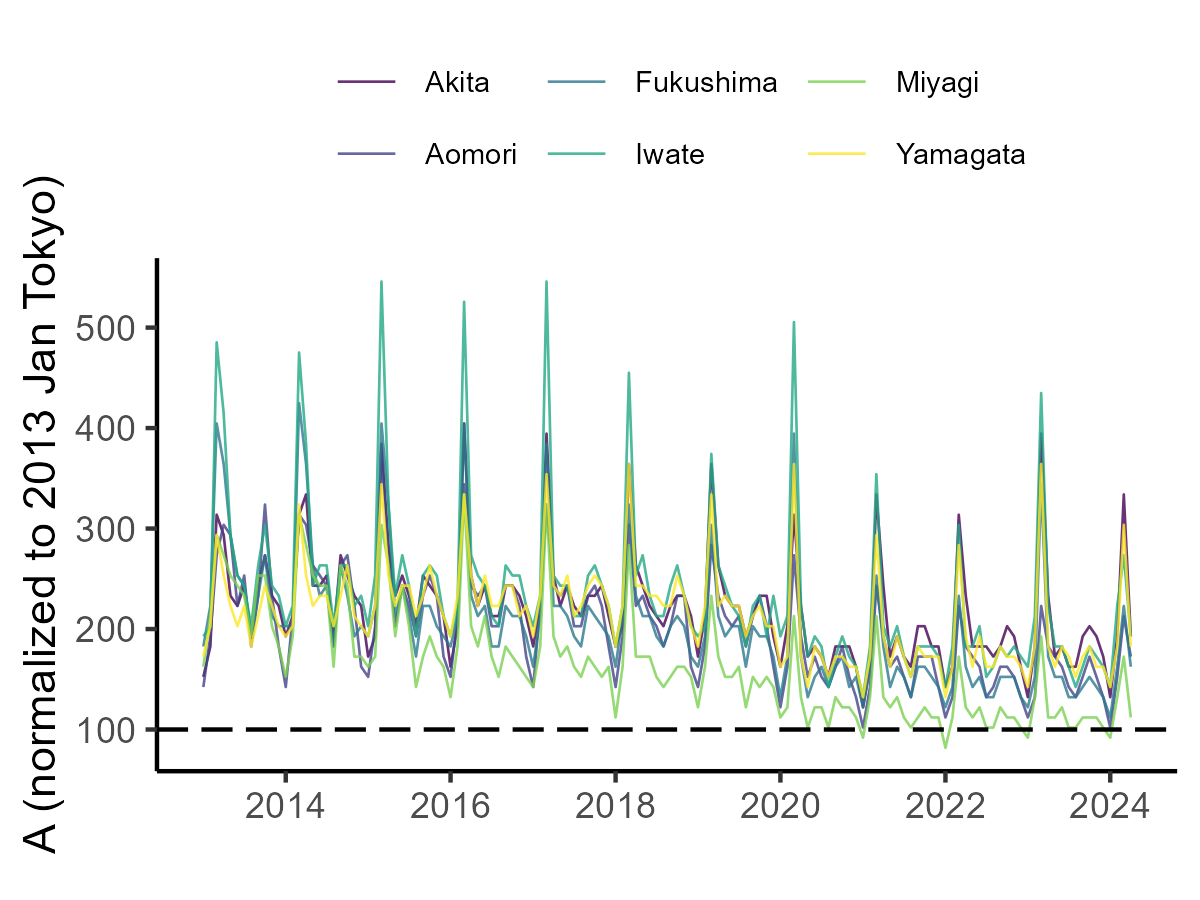
\includegraphics[width = 0.37\textwidth]
  {figuretable/matching_efficiency_month_aggregate_tohoku.png}
  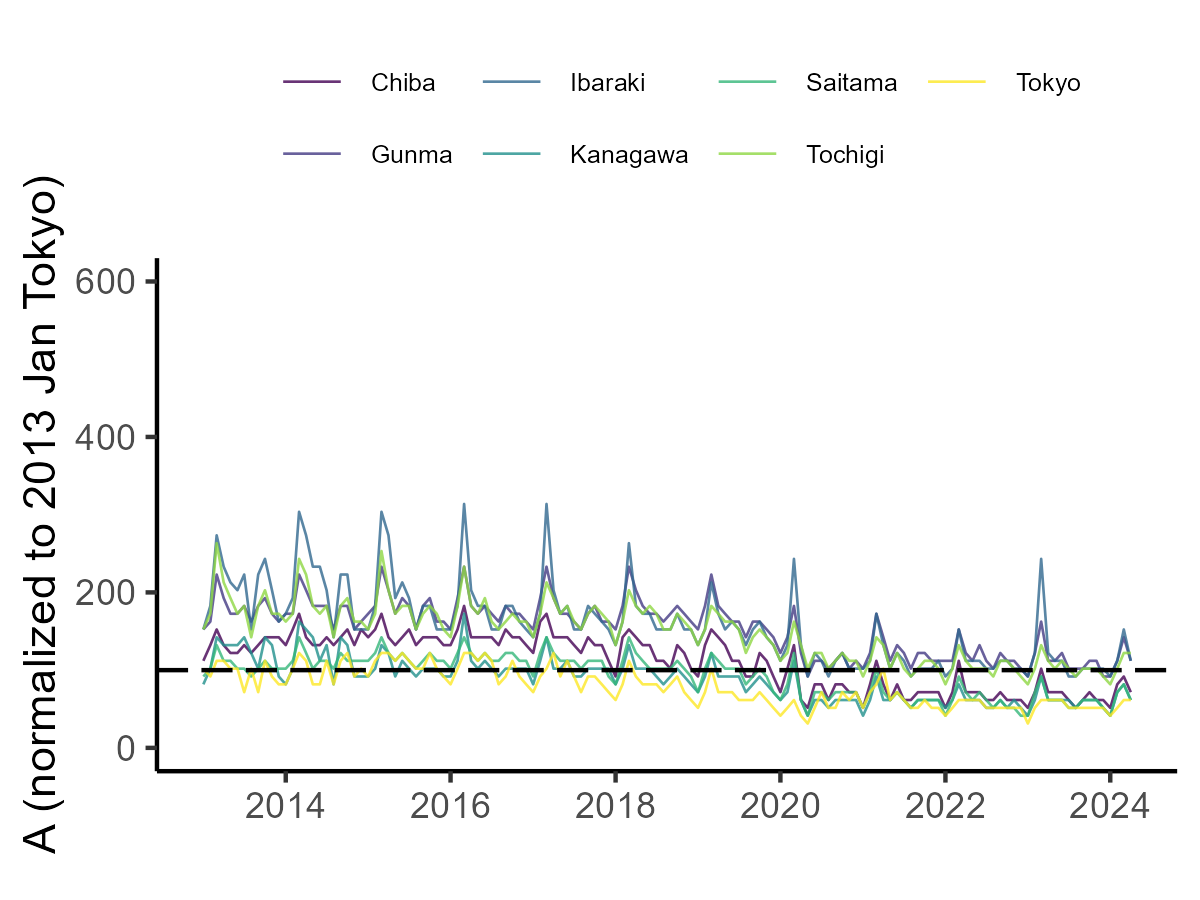
\includegraphics[width = 0.37\textwidth]
  {figuretable/matching_efficiency_month_aggregate_kanto.png}
  % \subfloat[Chubu]{\includegraphics[width = 0.37\textwidth]
  % {figuretable/matching_efficiency_month_aggregate_chubu.png}}
  % \\
  % \subfloat[Kansai]{\includegraphics[width = 0.37\textwidth]
  % {figuretable/matching_efficiency_month_aggregate_kansai.png}}
  % \subfloat[Chugoku]{\includegraphics[width = 0.37\textwidth]
  % {figuretable/matching_efficiency_month_aggregate_chugoku.png}}\\
  % \subfloat[Shikoku]{\includegraphics[width = 0.37\textwidth]
  % {figuretable/matching_efficiency_month_aggregate_shikoku.png}}
  % \subfloat[Kyusyu, Okinawa]{\includegraphics[width = 0.37\textwidth]
  % {figuretable/matching_efficiency_month_aggregate_kyushu.png}}
  % \caption{Month-level aggregate results 2012-2024}
  % \label{fg:month_part_and_full_time_matching_efficiency_prefecture_results} 
  \end{center}
  \footnotesize
  %Note: 
\end{figure} 
\end{frame}

\begin{frame}{Matching Elasticities: Tohoku and Kanto}
\begin{figure}[!ht]
  \begin{center}
  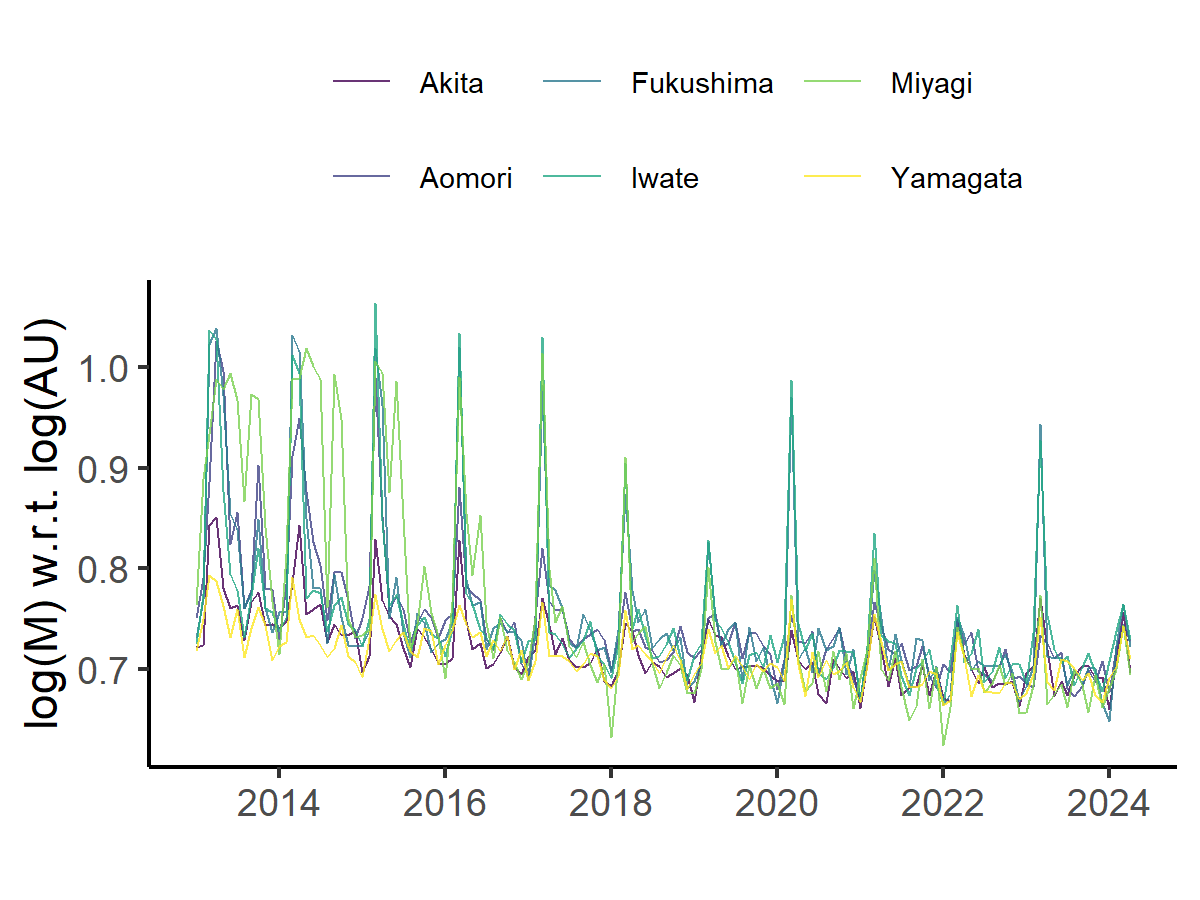
\includegraphics[width = 0.37\textwidth]
  {figuretable/elasticity_unemployed_month_aggregate_tohoku.png}
  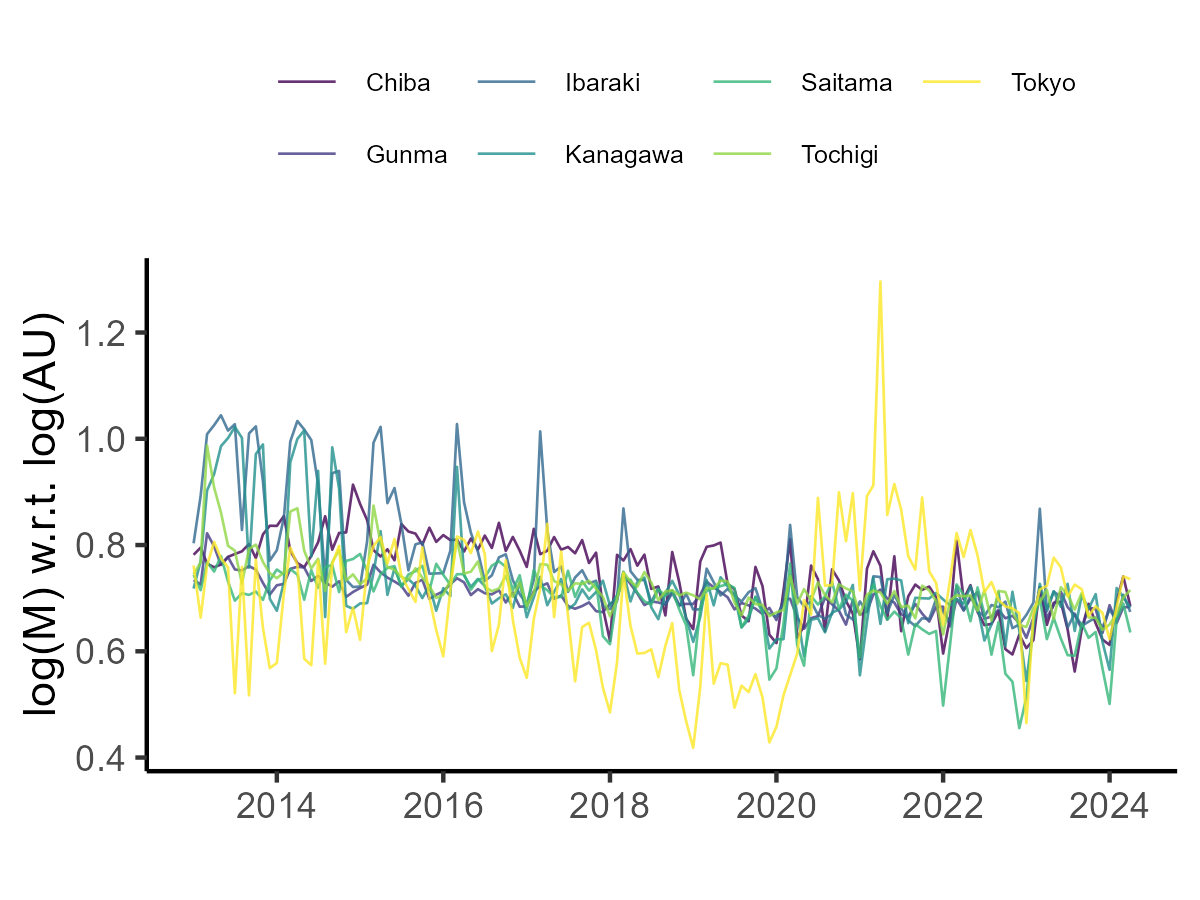
\includegraphics[width = 0.37\textwidth]
  {figuretable/elasticity_unemployed_month_aggregate_kanto.png}
  % \subfloat[Chubu]{\includegraphics[width = 0.37\textwidth]
  % {figuretable/elasticity_unemployed_month_aggregate_chubu.png}}
  % \\
  % \subfloat[Kansai]{\includegraphics[width = 0.37\textwidth]
  % {figuretable/elasticity_unemployed_month_aggregate_kansai.png}}
  % \subfloat[Chugoku]{\includegraphics[width = 0.37\textwidth]
  % {figuretable/elasticity_unemployed_month_aggregate_chugoku.png}}\\
  % \subfloat[Shikoku]{\includegraphics[width = 0.37\textwidth]
  % {figuretable/elasticity_unemployed_month_aggregate_shikoku.png}}
  % \subfloat[Kyusyu, Okinawa]{\includegraphics[width = 0.37\textwidth]
  % {figuretable/elasticity_unemployed_month_aggregate_kyushu.png}}
  % \caption{Month-level aggregate results 2012-2024}
  % \label{fg:month_part_and_full_time_elasticity_unemployed_month_aggregate_prefecture_results} 
  \end{center}
  \footnotesize
  %Note: 
\end{figure} 
\begin{itemize}
    \item Kanto vs Tohoku
\end{itemize}
\end{frame}

\begin{frame}{Mismatch across prefectures}
\begin{itemize}
    \item TBA
\end{itemize}
\end{frame}

\begin{frame}{Mismatch across industries}
\begin{itemize}
    \item TBA
\end{itemize}
\end{frame}

\begin{frame}{Summary of short time trends}
    \begin{itemize}
        \item Matching efficiency
        \item Matching elasticities
        \item Mismatch across prefectures
        \item Mismatch across industries
    \end{itemize}
\end{frame}

\begin{frame}{Conclusion and Future work}
    \begin{itemize}
      \item Contributions and Findings
      \begin{itemize}
          \item Nonparametric approach and its finite sample performance
          \item Compute nonparametric mismatch index.
          \item Matching efficiency decreases and is driven by full-time one
          \item Mismatch is large (=0.9)
      \end{itemize}
      \item Future work
      \begin{itemize}
          \item Interesting counterfactual
          \item Endogeneity care formally (Imbens and Newey (2009))
      \end{itemize}
    \end{itemize}
\end{frame}

\end{document}